\chapter{Existing solutions}
In this chapter we discuss currently available applications which have similar goals to our application.
First we introduce the applications.
After that we form use cases by which we will compare the applications.
Finally, we describe how each application covers the use cases.

\section{Overview of existing applications}
Now we will introduce the currently available applications.

\subsection*{Allergy Menu}
  Allergy menu\footnote{\url{https://allergymenu.uk}  \label{fnlabel}} allows a restaurant employee to maintain a mobile accessible and up-to-date menus that customers can tailor to their food preferences.
  
  A restaurant employee first creates a new menu and adds categories to it, e.g. "Starters" or "Desserts".
  Dishes are then added to each category of the menu.
  A dish contains allergen information as well as flags whether it is suitable for vegans and vegetarians.
  The restaurant employee can also add calories to the dish.

  When a restaurant employee wants to change something in a dish, they can create a copy of the dish which is hidden on the published menu.
  After they finish changes, the dish can be marked as "live", making it appear on the menu with updated content. 

  A dish can optionally contain internal notes, with the ability to upload photographs of products used within the dish.
  The application sends and e-mail regularly to review a menu with all the allergy information.
  An existing menu can be imported to the application in the CSV format.
  Allergy Menu provides an API for food suppliers, allowing them to sync menu information directly into the application without manual intervention.
  
  A guest can interact with a published menu by choosing what allergens they want to avoid.
  The application then filters out items of the menu to meet the guest's preferences.
  A guest can also select an option that they are either a vegan or vegetarian.
  
  A unique restaurant code is used to identify restaurants. 
  This is what guests enter into the application when they want to browse a menu.
  A guest can also find a restaurant which uses the application on a map.

  \newpage

  \begin{figure}[h]
    \centering
    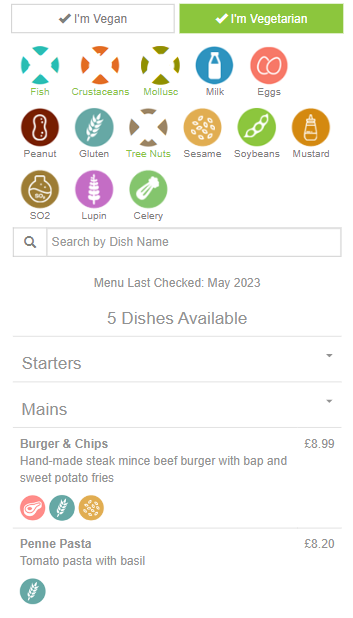
\includegraphics[height=12cm]{master-thesis/img/existing-applications-screenshots/allergy_menu_screenshot}
    \caption{The Allergy Menu application}
  \end{figure}
% end of \subsection

\subsection*{Allergen Checker}
  Allergen Checker\footnote{\url{https://allergenchecker.co.uk/}  \label{fnlabel}} is an allergen management software which enables a restaurant employee to add allergen information to a menu.
  
  A menu is created in three steps.
  In the first step, the restaurant employee creates ingredients which are then stored in a database called the restaurant's "virtual food cupboard".
  During the second step, the restaurant employee creates dishes by specifying their ingredients.
  In the third step, the restaurant employee creates a menu by specifying its dishes.
  
  The application provides a pre-defined list of basic ingredients in its database.
  An ingredient has information about what allergen it contains and also what allergens it may contain. 
  The restaurant employee can also copy information from the ingredient's packaging which will be then displayed in a dish's description in the menu.
  
  Allergen Checker allows for categorizing of dishes and menus. 
  Categories are thought of as a file system for dishes and menus.
  This is convenient when the restaurant employee needs to search for a specific menu or dish.

  \begin{figure}[h]
    \centering
    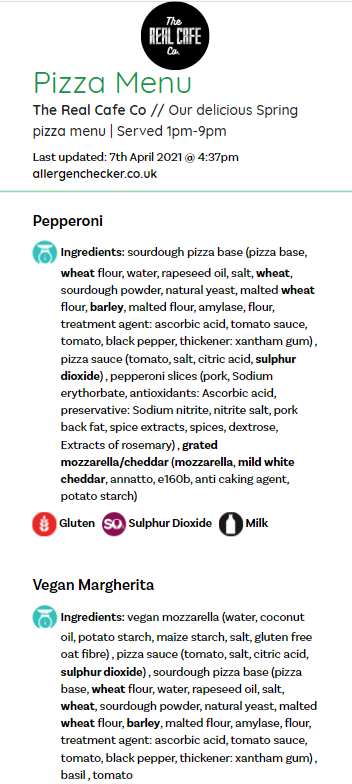
\includegraphics[height=12cm]{master-thesis/img/existing-applications-screenshots/allergen_checker_menu_screenshot}
    \caption{The Allergen Checker application}
  \end{figure}
% end of \subsection

\subsection*{BigZpoon Eagle}
  BigZpoon Eagle\footnote{\url{https://bigzpoon.com/nutrition-menus}  \label{fnlabel}} provides preference-based allergen and nutrition menus for \linebreak restaurants.
  It is a cloud-based SaaS solution which and two parts.

  One part is the consumer-facing website.
  It allows a restaurant's guest to set their dietary restrictions and nutritional goals.
  After this is done, a personalized menu is presented to the guest.
  Items of a menu are shown in three groups.
  There are items which are "Okay to eat", items which are "Okay to eat with modifications" and items which are "Not okay to eat".
  Items and ingredients which are not okay to eat are clearly marked in the item's detail.
  
  The application also supports online ordering of meals.
  The guest can select what they want to eat and choose different ingredients.
  The Eagle platform tries to recommend to the guest what they might want to order using a sort of artificial intelligence algorithm.
  The application also displays detailed nutritional information for the current state of the order and shows whether the guest's nutritional goals are met.

  The consumer-facing website sends analytical data to the backend portal application, which is the other part of the Eagle platform.
  It serves for restaurants to manage their online menus and see insights on how their customers are using the guest application.
  The portal application allows creating multi-location menus to show a different menu based on the restaurant's location.
  The restaurant employee can set up menu groups, categories and individual food items.
  A menu item can be disabled for a certain category, group or restaurant location.
  Creating a menu item involves adding all choices and their variations.
  A restaurant employee can manually create restaurant ingredients or choose from a pre-defined list of ingredients.

  \begin{figure}[h]
    \centering
    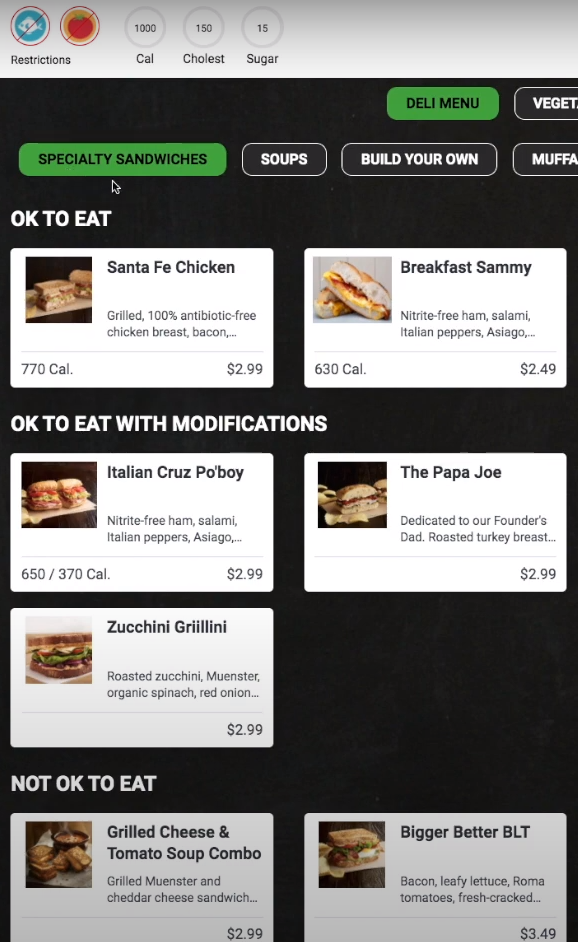
\includegraphics[height=12cm]{master-thesis/img/existing-applications-screenshots/bigzpoon_screenshot}
    \caption{The BigZpoon Eagle application}
  \end{figure}
% end of \subsection

\newpage

\subsection*{Menutech}
  Menutech\footnote{\url{https://menutech.com/en/restaurants}  \label{fnlabel}} provides automated allergen detection, menu translation and design templates for restaurants.
  
  A menu in the application consists of sections and sections contain dishes.
  A restaurant employee can create diets, dishes and recipes.
  A dish can have labels like gluten-free, vegetarian, spicy etc.
  Nutrition rating of a dish can be specified in three levels, from poor to high nutrition.
  A URL linking to more information about the product can be added to a dish.
  The application uses artificial intelligence to suggest items of a menu.
  When specifying allergens, a restaurant employee can copy allergens from existing similar dishes.

  A cover page can be added to a menu.
  A restaurant employee can set colors and font for a menu and the application also provides templates of menus with various styles.
  Translations can be also added to a menu.
  A guest can view a menu as a PDF file or as a mobile friendly version.

  \begin{figure}[h]
    \centering
    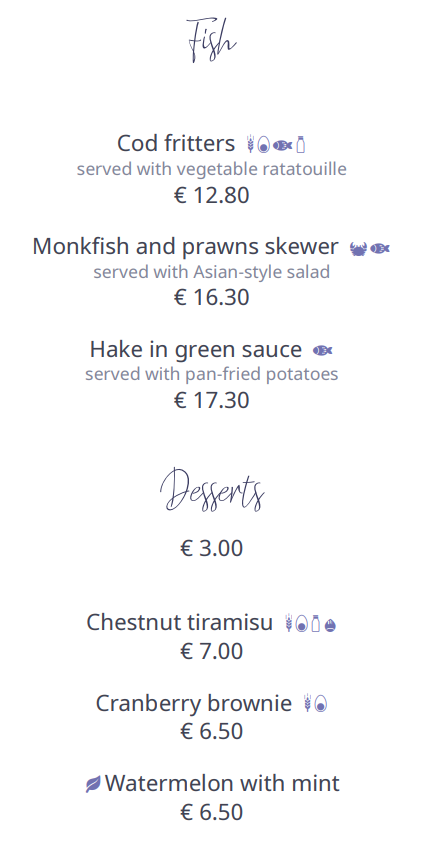
\includegraphics[height=12cm]{master-thesis/img/existing-applications-screenshots/menutech_screenshot}
    \caption{The Menutech application}
  \end{figure}
% end of \subsection

\subsection*{Menu Guide}
  Menu Guide\footnote{\url{https://menuguide.pro/}  \label{fnlabel}} is a tool used to maintain allergen and dietary information, and to share this information with restaurant staff and customers through interactive menus.

  A restaurant employee can create a menu from scratch or an existing menu can be uploaded from a website, pdf, CSV or some other supported formats. 
  A custom message which will be displayed upon opening a menu can be specified.
  The restaurant employee can choose from several menu design templates or apply custom styling using CSS.
  All menus have date of expiration for safety reasons.

  An item of a menu contains information like its name, price, calories and a list of ingredients as plain text.
  The restaurant employee clicks on allergen icons to specify allergens contained in the item.
  An item has more options for how it can contain an allergen. 
  Namely, it can surely contain the allergen, or it may or may not contain the allergen, or it may or may not contain traces of the allergen.
  When ingredients are inserted as text, the application automatically highlights ingredients in the text which contain allergens.
  Some allergens like nuts contain sub-allergens to choose from, e.g. almond or cashew.
  A food item can be marked as vegan, vegetarian or as gluten free etc.
  The restaurant employee can save commonly used menu items into a library for re-use in future. 

  The restaurant employee can create a link between two menus in a parent---child manner.
  When a parent menu is edited, changes are automatically propagated into its child menus.
  Deleting a parent menu will also delete all menus which are linked to it.

  A restaurant guest is able to select allergens and dietary options like being vegan or vegetarian.
  The application can filter or highlight menu items which do not correspond to the guest's selected preferences.
  It can also be set to remember the guest's preferences for future use.

  Menu Guide provides analytical insights like a daily breakdown of page views and the allergens and dietary preferences selected by diners.

  \begin{figure}[h]
    \centering
    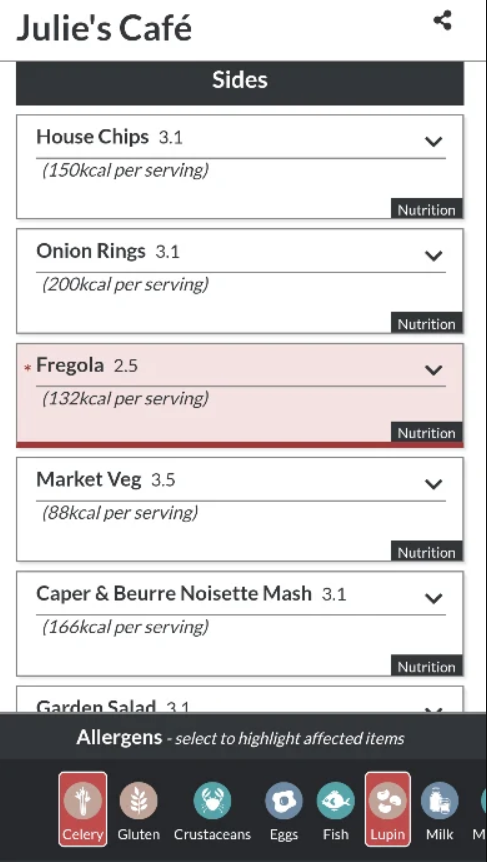
\includegraphics[height=12cm]{master-thesis/img/existing-applications-screenshots/menu_guide_screenshot}
    \caption{The Menu Guide application}
  \end{figure}
% end of \subsection
